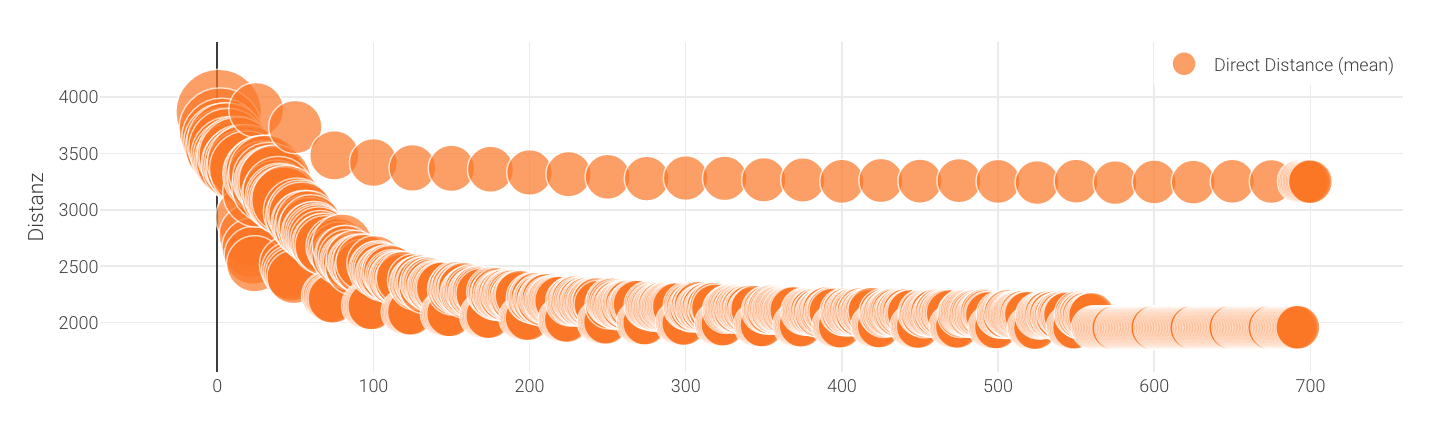
\includegraphics{assets/bubbles.png} \emph{A ``bubble'' plot, a type of
scatterplot where the circle sizes are variable}

Scatterplots and bubble plots allow you to plot data on two independent
axes.

\hypertarget{usage}{%
\subsection{Usage}\label{usage}}

Scatterplots can only be included as panels in \textbf{Dashboards}. See
Dashboard documentation for general tips on creating dashboard
configurations.

\begin{itemize}
\tightlist
\item
  Each chart panel is defined inside a \textbf{row} in a
  \texttt{dashboard-*.yaml} file.
\item
  Choose from panel types \texttt{scatter} and \texttt{bubble} in the
  dashboard configuration.
\item
  Standard title, description, and width fields define the frame.
\end{itemize}

\begin{center}\rule{0.5\linewidth}{0.5pt}\end{center}

\hypertarget{sample-dashboard.yaml-config-snippet}{%
\subsubsection{Sample dashboard.yaml config
snippet}\label{sample-dashboard.yaml-config-snippet}}

\begin{Shaded}
\begin{Highlighting}[]
\FunctionTok{layout}\KeywordTok{:}
\AttributeTok{  }\FunctionTok{row1}\KeywordTok{:}
\AttributeTok{    }\KeywordTok{{-}}\AttributeTok{ }\FunctionTok{type}\KeywordTok{:}\AttributeTok{ }\StringTok{\textquotesingle{}scatter\textquotesingle{}}
\AttributeTok{      }\FunctionTok{title}\KeywordTok{:}\AttributeTok{ }\StringTok{\textquotesingle{}Y vs. X\textquotesingle{}}
\AttributeTok{      }\FunctionTok{description}\KeywordTok{:}\AttributeTok{ }\StringTok{\textquotesingle{}a scatterplot\textquotesingle{}}
\AttributeTok{      }\FunctionTok{width}\KeywordTok{:}\AttributeTok{ }\DecValTok{3}
\AttributeTok{      }\FunctionTok{dataset}\KeywordTok{:}\AttributeTok{ }\StringTok{\textquotesingle{}*drt\_customer\_stats.csv\textquotesingle{}}
\AttributeTok{      }\FunctionTok{x}\KeywordTok{:}\AttributeTok{ }\StringTok{\textquotesingle{}iteration\textquotesingle{}}
\AttributeTok{      }\FunctionTok{usedCol}\KeywordTok{:}\AttributeTok{ }\KeywordTok{[}\AttributeTok{distance}\KeywordTok{]}
\AttributeTok{      }\FunctionTok{legendName}\KeywordTok{:}\AttributeTok{ }\KeywordTok{[}\StringTok{\textquotesingle{}Distance (mean)\textquotesingle{}}\KeywordTok{]}
\AttributeTok{      }\FunctionTok{xAxisName}\KeywordTok{:}\AttributeTok{ }\StringTok{\textquotesingle{}Iteration\textquotesingle{}}
\AttributeTok{      }\FunctionTok{yAxisName}\KeywordTok{:}\AttributeTok{ }\StringTok{\textquotesingle{}Distance, m\textquotesingle{}}
\AttributeTok{      }\FunctionTok{markerSize}\KeywordTok{:}\AttributeTok{ }\DecValTok{5}

\AttributeTok{    }\KeywordTok{{-}}\AttributeTok{ }\FunctionTok{type}\KeywordTok{:}\AttributeTok{ }\StringTok{\textquotesingle{}bubble\textquotesingle{}}
\AttributeTok{      }\FunctionTok{title}\KeywordTok{:}\AttributeTok{ }\StringTok{\textquotesingle{}Y vs. X\textquotesingle{}}
\AttributeTok{      }\FunctionTok{description}\KeywordTok{:}\AttributeTok{ }\StringTok{\textquotesingle{}a bubbley scatterplot\textquotesingle{}}
\AttributeTok{      }\FunctionTok{width}\KeywordTok{:}\AttributeTok{ }\DecValTok{2}
\AttributeTok{      }\FunctionTok{dataset}\KeywordTok{:}\AttributeTok{ }\StringTok{\textquotesingle{}*drt\_customer\_stats.csv\textquotesingle{}}
\AttributeTok{      }\FunctionTok{x}\KeywordTok{:}\AttributeTok{ }\StringTok{\textquotesingle{}iteration\textquotesingle{}}
\AttributeTok{      }\FunctionTok{y}\KeywordTok{:}\AttributeTok{ }\StringTok{\textquotesingle{}distance\_mean\textquotesingle{}}
\AttributeTok{      }\FunctionTok{bubble}\KeywordTok{:}\AttributeTok{ }\StringTok{\textquotesingle{}directDistance\textquotesingle{}}
\AttributeTok{      }\FunctionTok{factor}\KeywordTok{:}\AttributeTok{ }\DecValTok{100}
\AttributeTok{      }\FunctionTok{legendName}\KeywordTok{:}\AttributeTok{ }\KeywordTok{[}\StringTok{\textquotesingle{}Distance (mean)\textquotesingle{}}\KeywordTok{]}
\AttributeTok{      }\FunctionTok{markerSize}\KeywordTok{:}\AttributeTok{ }\DecValTok{5}
\AttributeTok{      }\FunctionTok{skipFirstRow}\KeywordTok{:}\AttributeTok{ }\CharTok{false}
\AttributeTok{      }\FunctionTok{xAxisName}\KeywordTok{:}\AttributeTok{ }\StringTok{\textquotesingle{}Iteration\textquotesingle{}}
\AttributeTok{      }\FunctionTok{yAxisName}\KeywordTok{:}\AttributeTok{ }\StringTok{\textquotesingle{}Distance, m\textquotesingle{}}
\end{Highlighting}
\end{Shaded}

\begin{center}\rule{0.5\linewidth}{0.5pt}\end{center}

\hypertarget{scatterplot-and-bubbleplot-properties}{%
\subsubsection{Scatterplot and bubbleplot
properties}\label{scatterplot-and-bubbleplot-properties}}

\textbf{dataset:} (Required) String. The filepath containing the data.
May include wildcards * and ?.

\textbf{x:} String. The column containing x-values.

\textbf{y:} String. The column containing y-values.

\textbf{bubble:} String. The column containing bubble size values.

\textbf{legendName:} Array of strings. Legend titles for each line. The
column names will be used if this is omitted.

\textbf{xAxisName/yAxisName:} Labels for the axes.
